\appendix
%\chapter*{Appendices}
   \nonumchapter{Appendices}


\section{ Code Snippets }
It should be noted that this Appendix only contains the main source code snippets and does not contain any of the code written for the data preprocessing steps or the Node.JS web app as there is too much code. For further insight please visit \href{https://github.com/SurveNet}{https://github.com/SurveNet}. 

\subsection{TensorFlow Training Script}
\begin{lstlisting}[language=python, frame=single]
import tensorflow as tf
import os, os.path
import pandas as pd
import time
import numpy as np
from numpy import ndarray
import skimage
from skimage import data, io, filters, transform, exposure
import random
from PIL import Image
import matplotlib
import matplotlib.pyplot as plt
%matplotlib inline

print('imported')

TRAINING_DIR = '/data/training'
TESTING_DIR = '/data/testing'

MODEL_PATH = '/output/trained_model.ckpt'
SAVE = '/output/'

# Define initial variables
batch_size = 100
num_class = 6
num_epochs = 20
image_size = 50 # in pixels, square assumed

################################################
'''
This function traverses throwe ach directory of training images
Two lists are made:
- The RGB image values are added to the images list
- For every photo in say the 'angry' directory of images, a 
corresponding label is added to the label list

'''
def load_data(TRAINING_DIR):
images = []
labels = []
directories = [d for d in os.listdir(TRAINING_DIR) 
if os.path.isdir(os.path.join(TRAINING_DIR, d))]
# Need to sort these because
# floyd hum jumbled up the order
directories = sorted(directories, key=int)

# Traverse through each directory and make a list
# of files names if they end in the PNG format
for d in directories:
label_directory = os.path.join(TRAINING_DIR, d)
file_names = [os.path.join(label_directory, f) 
for f in os.listdir(label_directory) 
if f.endswith(".png")]
#Traverse through each file, add the image data
# and label to the 2 lists
for f in file_names:
images.append(skimage.data.imread(f))
labels.append(int(d))

return images, labels

images, labels = load_data(TRAINING_DIR)

print('data read...')

'''
Shuffle the entire dataset and labels
'''

from sklearn.utils import shuffle
images, labels = shuffle(images, labels)

'''
This cell is  for converting to one hot

'''
num_images = len(images)
images = np.array(images, object)
labels = np.array(labels, dtype = np.int32)

_labels = np.zeros((num_images, num_class))
_labels[np.arange(num_images), labels] = 1.0
labels = _labels


'''
Plot an image and label  of the same indices after
being randomly shuffled to confirm they
represent the same expression
'''
print('Angry = 0, fear = 1, happy = 2, 
neutral = 3, sadness = 4, suprise = 5')

plt.axis('off')
plt.imshow(images[9], cmap='gray')
plt.subplots_adjust(wspace=0.1)
plt.show()


print(labels[9])
 
################################################
'''
import test data and labels
'''
def load_test_data(TESTING_DIR):
test_images = []
test_labels = []
directories = [d for d in os.listdir(TESTING_DIR) 
if os.path.isdir(os.path.join(TESTING_DIR, d))]
# Need to sort these because
# floyd hum jumbled up the order
directories = sorted(directories, key=int)

# Traverse through each directory and make a list
# of files names if they end in the PNG format
for d in directories:
label_directory = os.path.join(TESTING_DIR, d)
file_names = [os.path.join(label_directory, f) 
for f in os.listdir(label_directory) 
if f.endswith(".png")]
#Traverse through each file, add the image data
# and label to the 2 lists
for f in file_names:
test_images.append(
transform.resize(skimage.data.imread(f),
 (image_size, image_size) ) )
test_labels.append(int(d))

return test_images, test_labels

test_images, test_labels = load_test_data(TESTING_DIR)

print('Imported...')

#Shuffle data and labels
test_images, test_labels = shuffle(test_images, test_labels)


'''
This cell is  for converting  to one hot
''' 

num_images = len(test_images)
test_images = np.stack( test_images )
test_labels = np.array( test_labels, dtype = np.int32 )

_test_labels = np.zeros((num_images, num_class))
_test_labels[np.arange(num_images), test_labels] = 1.0
test_labels = _test_labels

print('converted...')

print('Angry = 0, fear = 1, happy = 2, 
neutral = 3, sadness = 4, suprise = 5')

plt.axis('off')
plt.imshow(test_images[5], cmap = 'gray')
plt.subplots_adjust(wspace=0.1)
plt.show()

print(test_labels[5])

#######################################
'''
This cell is for image downsampling and transformation
This is on the fly to resize the images to a 50x50 size
'''

print('Down scaling train images...')
images = [transform.resize(image, (50, 50)) 
	for image in images]

# print('equalizing exposure...')
# images = [exposure.equalize_adapthist(image,
		 clip_limit=0.0001)for image in images50]

print('Images Downscaled...')

'''
This cell is for initializing variables for the tensorflow 
session and placeholders for holding the data.
'''

# Initialize placeholders 
x = tf.placeholder(dtype = tf.float32, shape 
= [None, 50, 50], name='X_placeholder')
y = tf.placeholder(dtype = tf.float32, shape= 
[None, num_class],name="Y_placeholder")
is_training = tf.placeholder( dtype = tf.bool, shape = 
(), name = "is_training" )

#define variables for dropout
keep_rate = .8
keep_prop = tf.placeholder(tf.float32)
print('initialized')

#################################################

'''
Network stucture using tensorflow slim to easily 
implement layers 

'''
import tensorflow.contrib.slim as slim

def convolutional_network_v2(x, is_training):
net = tf.reshape(x, shape=[-1, 50, 50, 1]) # add channel dim

with slim.arg_scope( [ slim.conv2d ],
padding = "SAME",
activation_fn = tf.nn.relu,
stride = 1,
weights_initializer = tf.truncated_normal_initializer
(stddev=0.01),
weights_regularizer = slim.l2_regularizer(0.0005),
normalizer_fn = slim.batch_norm,
normalizer_params = {'scale' : True, 'trainable' : False, 
'is_training' : is_training }):

net = slim.conv2d(net, 32, 3)
net = slim.conv2d(net, 64, 3)
net = slim.conv2d(net, 64, 3)
net = slim.max_pool2d(net, 3, stride = 1 )
net = slim.conv2d(net, 96, 3)
net = slim.conv2d(net, 96, 3)
net = slim.max_pool2d( net, 2, stride = 2)

net = slim.conv2d(net, 128, 3)
net = slim.conv2d(net, 128, 3)
net = slim.max_pool2d( net, 2, stride = 2)

net = slim.conv2d(net, 128, 3)
net = slim.conv2d(net, 128, 3)
net = slim.max_pool2d(net, 2, stride = 2)

net = slim.conv2d(net, 128, 3)
net = slim.max_pool2d(net, 2, stride = 1)

net = slim.dropout(net, keep_prob = keep_rate,
 is_training = is_training )

with slim.arg_scope([slim.fully_connected ], 
weights_regularizer = slim.l2_regularizer(0.0005)):
net = slim.flatten(net)
output = slim.fully_connected(net, num_class,
			 activation_fn = None)
prediction = tf.nn.softmax(output, name = "Prediction" ) 

return output, prediction

#####################################################
'''
Shuffle the batches on the fly 

'''

def randomize(batch_x, batch_y):
batch_x, batch_y = shuffle(batch_x, batch_y)
return batch_x, batch_y


#####################################################



def train_network(x):
output, prediction = convolutional_network_v2(x, is_training)

#Use Softmax cross entropy for the loss function
loss = tf.reduce_mean(tf.nn.softmax_cross_entropy_with_logits
(labels = y, logits = output))
total_losses = tf.losses.get_total_loss( 
add_regularization_losses=True ) + loss

update_ops = tf.get_collection(tf.GraphKeys.UPDATE_OPS)
with tf.control_dependencies(update_ops):
train_op = tf.train.AdamOptimizer( learning_rate=0.002 )
.minimize( total_losses )

# Use these to print out predicted and actual labels
pred_class = tf.argmax(prediction,1)
label_class = tf.argmax(y, 1)

#Accuracy Metric
correct = tf.equal(tf.argmax(prediction,1),  tf.argmax(y, 1))
acc = tf.reduce_mean(tf.cast(correct, 'float'))

with tf.Session() as sess:
sess.run(tf.global_variables_initializer())
saver = tf.train.Saver()

time_full_start = time.clock()
print("RUNNING SESSION...")
for epoch in range(num_epochs):
train_batch_x = []
train_batch_y = []
epoch_loss= 0
epoch_total_loss = 0
accuracy = 0
time_epoch_start = time.clock()
i = 0
number_of_batches = 0

#For all images in the DS, batch into sizes of 100
while i < len(images):
start = i
end = i + batch_size
train_batch_x = images[start:end]
train_batch_y = labels[start:end]

#Randomize the batches even more
train_batch_x, train_batch_y = randomize(train_batch_x,
 train_batch_y)

#Feed batches into tensorflow
op, ac, loss_value, total_loss_value, 
pred_classes, label_classes =  sess.run([train_op, acc, loss,
 total_losses, pred_class, label_class ],
feed_dict={x: train_batch_x, y: train_batch_y,
 is_training : True})

epoch_loss += loss_value
epoch_total_loss += total_loss_value
accuracy += ac
i += batch_size
number_of_batches += 1

accuracy /= number_of_batches       
print('Epoch:', epoch+1, 'total loss: ', epoch_total_loss  ,'
 loss: ', epoch_loss ,' acc: {:%}'.format(accuracy))

time_epoch_end = time.clock()
print('Time elapse: ', time_epoch_end - time_epoch_start)

time_full_end = time.clock()
print('Full time elapse:', time_full_end - time_full_start)

if epoch_loss < 100:
save_path = saver.save(sess, MODEL_PATH)
print("Model saved in file: " , save_path)

print('Accuracy:', acc.eval({x: test_images, y: test_labels,
 is_training : True }))
#############################################

train_network(x)
\end{lstlisting}


\subsection{TensorFlow Flask API}

\begin{lstlisting}[language=python, frame=single]
import numpy as np 
import os as os, os.path
import sys
import re
# sys.path.append(os.path.abspath('./model'))
from scipy.misc.pilutil import imsave, imread, imresize
from PIL import Image
from flask import (Flask, request, g, redirect, url_for, 
abort, Response, jsonify)
from flask_cors import CORS, cross_origin
import base64
import tensorflow as tf

"""
Import all the dependencies you need to load the model, 
preprocess your request and postprocess your result
"""
app = Flask(__name__)
CORS(app) # needed for cross-domain requests
app.config['CORS_HEADERS'] = 'Content-Type'
MODEL_PATH = os.getcwd() + '/data/'

os.environ['TF_CPP_MIN_LOG_LEVEL'] = '3' 

sess = tf.Session('', tf.Graph())
with sess.graph.as_default():       
saver = tf.train.import_meta_graph(MODEL_PATH +
 "trained_model.ckpt.meta")
saver.restore(sess, MODEL_PATH + "trained_model.ckpt")

# Get pointers to relevant tensors in graph
graph = tf.get_default_graph()
x = graph.get_tensor_by_name("X_placeholder:0") 
y = graph.get_tensor_by_name("Y_placeholder:0")
is_training = graph.get_tensor_by_name( "is_training:0" )
prediction = graph.get_tensor_by_name( "Prediction:0" )


def data_preprocessing(data):
imgstr = re.search(b'base64,(.*)',data).group(1)
with open('output.jpg','wb') as output:
output.write(base64.b64decode(imgstr))

# Every incoming POST request will run the `evaluate` method
@app.route('/api', methods=["POST"])
@cross_origin()
def evaluate():

imageData = request.get_data()
# CODE FOR DATA PREPROCESSING
data_preprocessing(imageData)
print('1: Image was converted')

image = Image.open('output.jpg')
image = image.convert('L')
image = image.resize((50, 50), Image.ANTIALIAS)
print('Resized and Grayscaled Image') 

image = np.expand_dims(np.array(image), axis = 0)
classification = sess.run(prediction, feed_dict = 
{x: image, is_training : True})   
classes = np.argmax( classification, axis = 1 )

res = 'undefined'
if   classes[0] == 0:
print('Predicted: Angry')
res = 'Angry'
elif classes[0] == 1:
print('Predicted: Fear')
res = 'Fear'
elif classes[0] == 2:
print('Predicted: Happy')
res = 'Happy'
elif classes[0] == 3:
print('Predicted: neutral')
res = 'Neutral'
elif classes[0] == 4:
print('Predicted: sad')
res = 'Sad'
elif classes[0] == 5:
print('Predicted: Suprised')
res = 'Suprised'

return jsonify(res)
@app.route('/api', methods=["GET"])
def api():

return 'Get Request Recieved...'

# Load the model and run the server
if __name__ == "__main__":
print(("* Loading model and starting Flask server..."
"please wait until server has fully started"))
app.debug = True
app.run(host='0.0.0.0')

\end{lstlisting}


\section{Screen shots}

\subsection{Single Inference with Trained Model}

\begin{figure}[ht]
	\begin{center}
		\advance\leftskip-3cm
		\advance\rightskip-3cm
		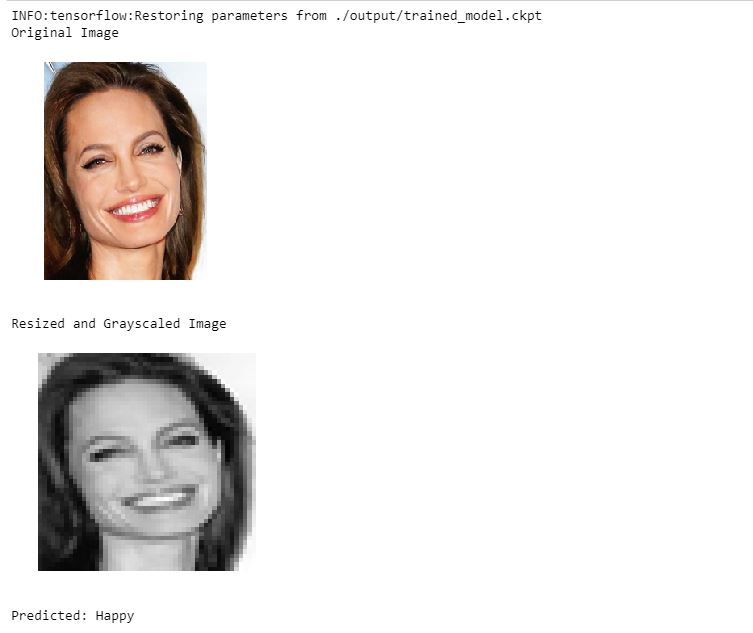
\includegraphics[keepaspectratio=true,scale=1]{__resources/Appendix/single.jpg}
		\caption{Single Inference with Random Google Image in Jupyter Notebook}
		\label{ui}
	\end{center}
\end{figure}

\newpage
\subsection{Web Application}

\begin{figure}[ht]
	\begin{center}
		\advance\leftskip-3cm
		\advance\rightskip-3cm
		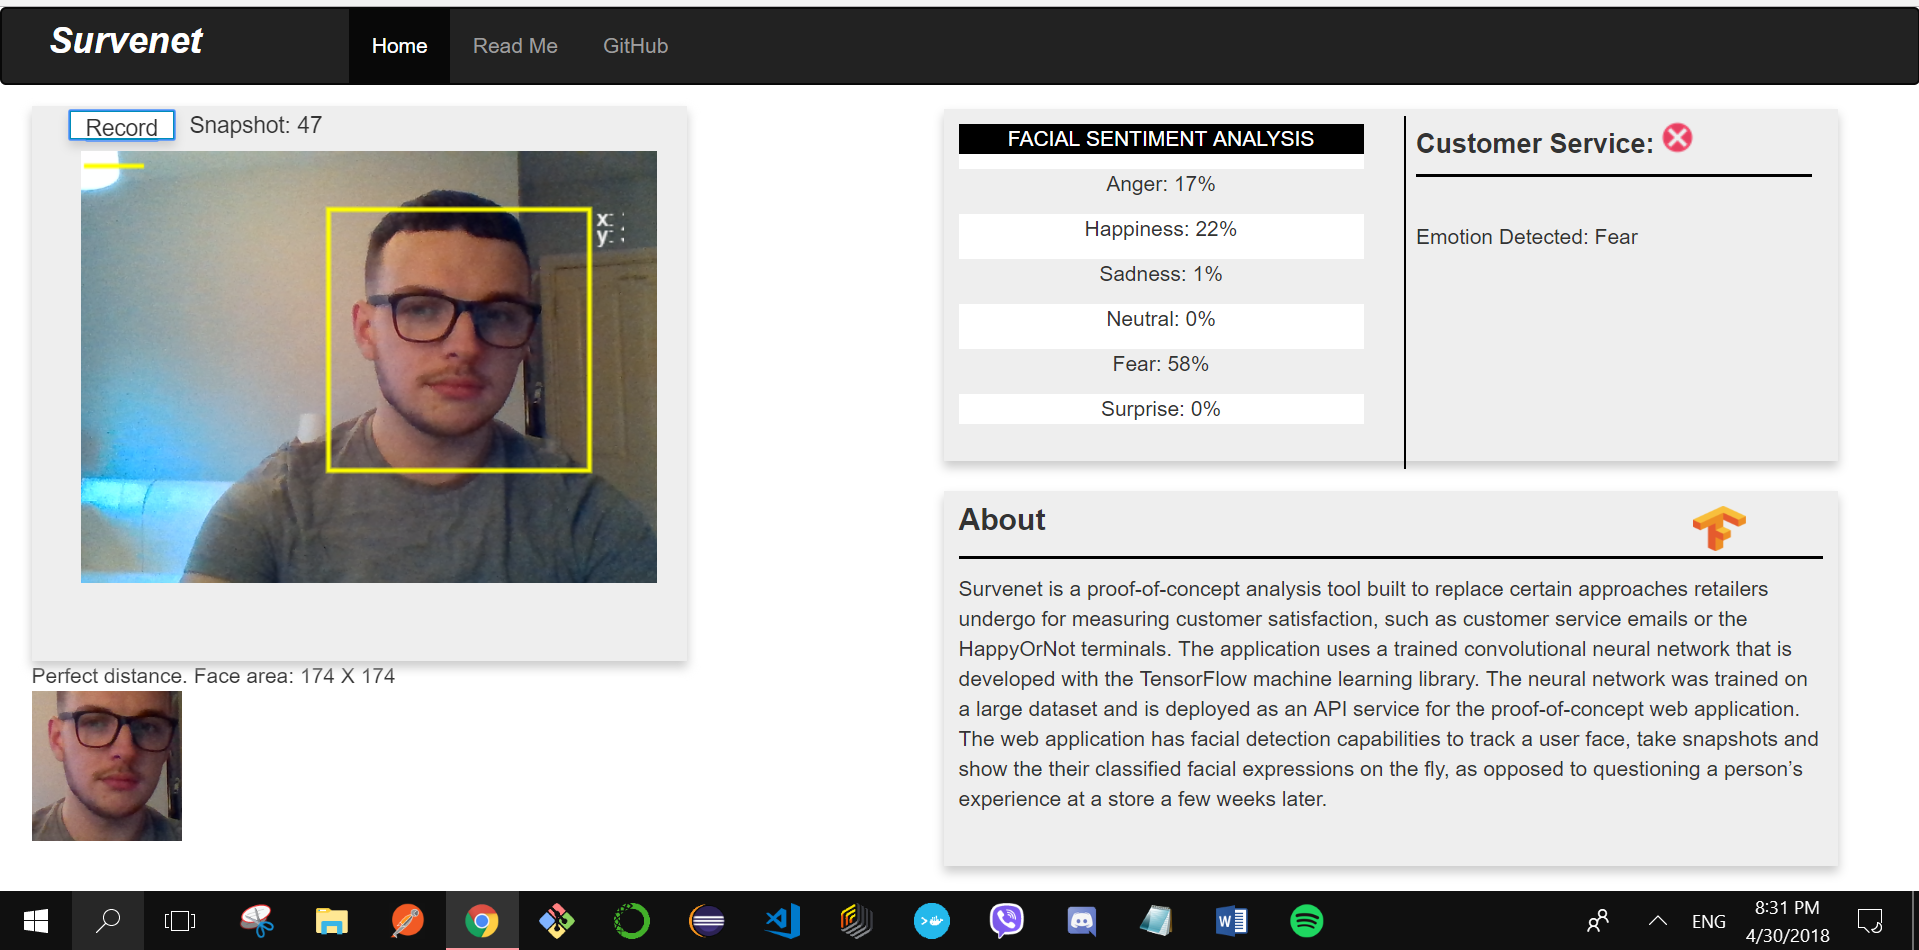
\includegraphics[keepaspectratio=true,scale=.3]{__resources/Appendix/screenshot.png}
		\caption{Screen Shot of Web Application}
		\label{screenshot}
	\end{center}
\end{figure}

\subsection{QR Code for Web Application}

\begin{figure}[ht]
	\begin{center}
		\advance\leftskip-3cm
		\advance\rightskip-3cm
		
\includegraphics[keepaspectratio=true,scale=.06]{__resources/Appendix/frame.png}
		\caption{QR Code for Survenet - Scan to View Application}
		\label{qr}
	\end{center}
\end{figure}

\newpage